\documentclass[12pt, twoside]{article}
\usepackage[francais]{babel}
\usepackage[T1]{fontenc}
\usepackage[latin1]{inputenc}
\usepackage[left=6mm, right=1cm, top=1cm, bottom=6mm]{geometry}
\usepackage{float}
\usepackage{graphicx}
\usepackage{array}
\usepackage{multirow}
\usepackage{amsmath,amssymb,mathrsfs}
\usepackage{soul}
\usepackage{textcomp}
\usepackage{eurosym}
 \usepackage{variations}
\usepackage{tabvar}

\begin{document}


\section*{\center{Devoir maison 8}}

\textit{Devoir � rendre sur feuille double grand format petits carreaux pour le
\ul{samedi 14 mars 2009}.}



\subsection*{Exercice 1}

\begin{enumerate}
  \item Tracer un triangle $ABC$ tel que $AC=12$cm,
  $BC=11$cm et $AB=14$cm.
  \item Tracer un triangle $EDF$ semblable au pr�c�dent tel que $DE=6$cm
  (justifier votre construction).
\end{enumerate}

\subsection*{Exercice 2}

Soit $ABCD$ un carr�. On place sur les c�t�s les points $M$, $N$, $P$ et $Q$
tels que: $AM=BN=CP=DQ$.

\begin{center}
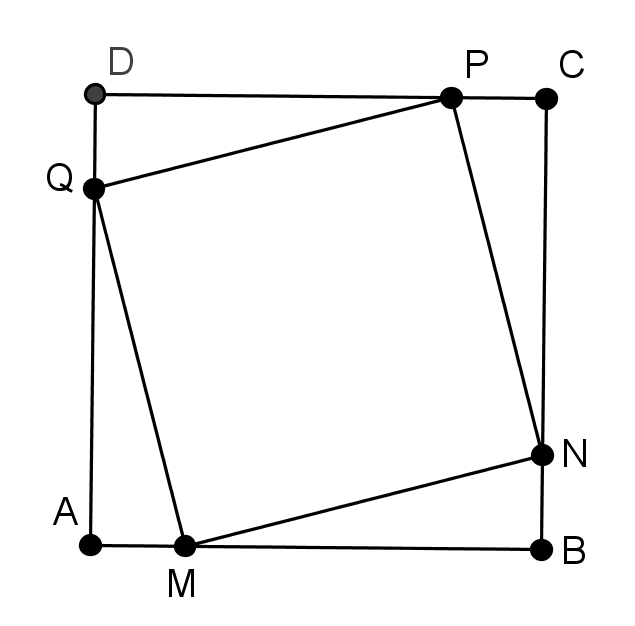
\includegraphics[width=4cm]{images/ex2.png}
\end{center}

\begin{enumerate}
  \item Faire la figure avec $AB=6cm$ et $AM=1cm$.
  \item D�montrer que $AMQ$ et $BNM$ sont isom�triques.
  \item Coder sur la figure toutes les �galit�s d'angles et de longueurs que
  l'on d�duit (justifier rapidement).
  \item Quels autres triangles leur sont isom�triques (justifier rapidement).
  \item D�montrer que $MNPQ$ est un losange.
  \item $MNPQ$ est-il un carr�?
\end{enumerate}



 \subsection*{Exercice 3}

$ABC$ est un triangle isoc�le de base $[BC]$ tel que $\widehat{BAC}=36$�. La
bissectrice de l'angle $\widehat{B}$ coupe $[AC]$ en $D$.
\begin{enumerate}
  \item D�montrer que les triangles $ABC$ et $BDC$ sont de m�me forme et que
  les triangles $ADB$ et $DBC$ sont isoc�les.
  \item La bissectrice de l'angle $\widehat{BDC}$ coupe $(BC)$ en $E$.
  D�montrer que les triangles $CDE$ et $DBC$ sont de m�me forme et que les
  triangles $BED$ et $CDE$ sont isoc�les.
  \item On pose $BC=1$ et $AC=x$.
  \begin{enumerate}
    \item D�montrer que $AD=1$.
    \item Calculer $DC$, $DE$, $BE$ et $EC$ en fonction de $x$.
    \item D�montrer que $(DE)$ est parall�le � $(AB)$.
    \item En d�duire que $x$ est solution de l'�quation: $x^{2}-x-1=0$ et
    donner la valeur exacte de $x$.
  \end{enumerate}
  \end{enumerate}
\end{document}
